
\documentclass[12pt]{article}
 
\usepackage[utf8]{inputenc}
\usepackage{hyperref}
\usepackage[margin=0.8in]{geometry} 
\usepackage{amsmath,amsthm,amssymb}
\usepackage{natbib}
\usepackage{subcaption}
\usepackage{biblatex}
\addbibresource{ref.bib}
\usepackage{eurosym}
\usepackage{lmodern}
\usepackage{tcolorbox}
\usepackage{graphicx}
\usepackage{subfig}
\usepackage{pgfplots}
\usepgflibrary{shapes}

\usepackage{pythonhighlight}
\usepackage{pgfplots}
\pgfplotsset{compat=1.14}

\date{}
\begin{document}

\pgfmathdeclarefunction{gauss}{2}{%
  \pgfmathparse{1/(#2*sqrt(2*pi))*exp(-((x-#1)^2)/(2*#2^2))}%
}

 
% ////////////////////////////////////////////////////////////
%                         Info begins
% ////////////////////////////////////////////////////////////

\section*{\textbf{Code journal: Numerical Derivative Visualization}}

02.01.2022, \textit{Mariana Ávalos Arce}

\subsection*{The Derivative of A Function}

The derivative of a function $f(x)$, usually called $f'(x)$, is defined as the following limit:

\begin{equation}
    f'(x) = \lim_{h\to0} \frac{f(x+h) - f(x)}{h}
\end{equation}

Where the term \textit{limit as h approaches 0} means \textbf{the value h is getting closest to zero as h becomes arbitrarily small}, even if the expression in question is unsolvable exactly as h = 0. There exists also a geometric definition that states that \textbf{a derivative $f'(x)$ is the value of the slope of the tangent line at x}, and this can be represented in a Cartesian plane given an example: say the function $f(x)$ is a curve plotted below, and we grab two arbitrary points in the x axis: $x$ and $x+h$, where $h$ is the \textbf{increment} from $x$ to arrive at $x+h$. Now, at these two points, we can evaluate the function $f(x)$ and get, for $x$ a value of $f(x)$, and for $x+h$ a value of $f(x+h)$ in the y axis, which is what we see below.

\begin{center}

\begin{tikzpicture}

    \begin{axis}[
  no markers, domain=0:8, samples=100,
  axis lines*=middle, xlabel=$x$, ylabel=$y$,
  every axis y label/.style={at=(current axis.above origin),anchor=south},
  every axis x label/.style={at=(current axis.right of origin),anchor=west},
  height=5cm, width=12cm,
  xtick=\empty, ytick=\empty,
  enlargelimits=false, clip=false, axis on top,
  %grid = major
  ]
        \addplot[very thick,cyan!50!black] {gauss(4,1)};
        
    \end{axis}
    \draw[dashed] (4.3,2.63) -- (4.3,0) node[below] {$x$};
    \draw[dashed] (4.3,2.63) -- (0, 2.63) node[left] {$f(x)$};
    
    \draw[dashed] (5.5,3.35) -- (5.5,0) node[below] {$x+h$};
    \draw[dashed] (5.5,3.35) -- (0,3.35) node[left] {$f(x+h)$};
    
    \draw [<->, ultra thick, color=black] (4.3,0.17) -- (5.5,0.17) node[midway,above] {$h$};
    \draw [--, ultra thick, color=black] (4.0,2.43) -- (5.7,3.45) node[right] {$a$};
\end{tikzpicture}
\end{center}

Line $a$ is a secant line since it crosses the function $f(x)$ twice, and we can calculate the slope of line $a$ as:

\begin{equation}
    m = \frac{y_2 - y_1}{x_2 - x_1} = \frac{f(x+h) - f(x)}{x + h - x} = \frac{f(x+h) - f(x)}{h}
\end{equation}

In this way, the ratio $\frac{f(x+h) - f(x)}{h}$ where $h$ is an arbitrary increment, would represent the slope of a secant line to $f(x)$. However, if we allow $h$ to get very small and close to 0, the line $a$ becomes a \textbf{tangent line of $f(x)$}, and the ratio $\frac{f(x+h) - f(x)}{h}$ where $h$ is very small becomes the \textbf{slope of a tangent line}, or the derivative. In other words, the expression in Eq. (1) simply says that when h approaches a value very close to 0, the function $\frac{f(x+h) - f(x)}{h}$ is the \textbf{slope of the tangent line of $f(x)$ at point x}. The ratio $\frac{f(x+h) - f(x)}{h}$, \textbf{if h was infinitesimal or very small} (for a larger $h$ would mean the slope of a \textit{secant line}), would be the same as calculating a the slope of a line (\textit{tangent} to $f(x)$), commonly known as $\frac{y_2 - y_1}{x_2 - x_1}$ and expressed below in Eq. (2). Thus, if we take the limit of the ratio $\frac{f(x+h) - f(x)}{h}$ when h is similar to 0, it computes \textbf{the slope of the tangent line at every point x of $f(x)$}, known as \textbf{the derivative}.
\\

Now, in order to visualize this, we need this ratio in Eq. (2) and a value of $h$ that is considerably small, so that we can evaluate this expression at every value of $x$ and get the slopes of tangent lines of $f(x)$ at every value of $x$. If we plot all these slopes of the different $x$ values of a definite domain as points ($x$, $\frac{f(x+h) - f(x)}{h}$), what we are actually plotting is \textbf{the derivative of function $f(x)$}. The example function for this plot will be a $sin(x)$ function, with the value of $h$ being h = 0.05, and the domain being ${x \in \mathbb{R} | 0 \leq x \leq 6\pi}$. In practice, the smallest $h$ is set, the more exact the derivative plot will be, in this case, if $h$ was instead set to h = 0.00001, the plot (black crosses) would get closer to the exact derivative function $f'(x) = cos(x)$.

\begin{figure}[ht]
    \centering
    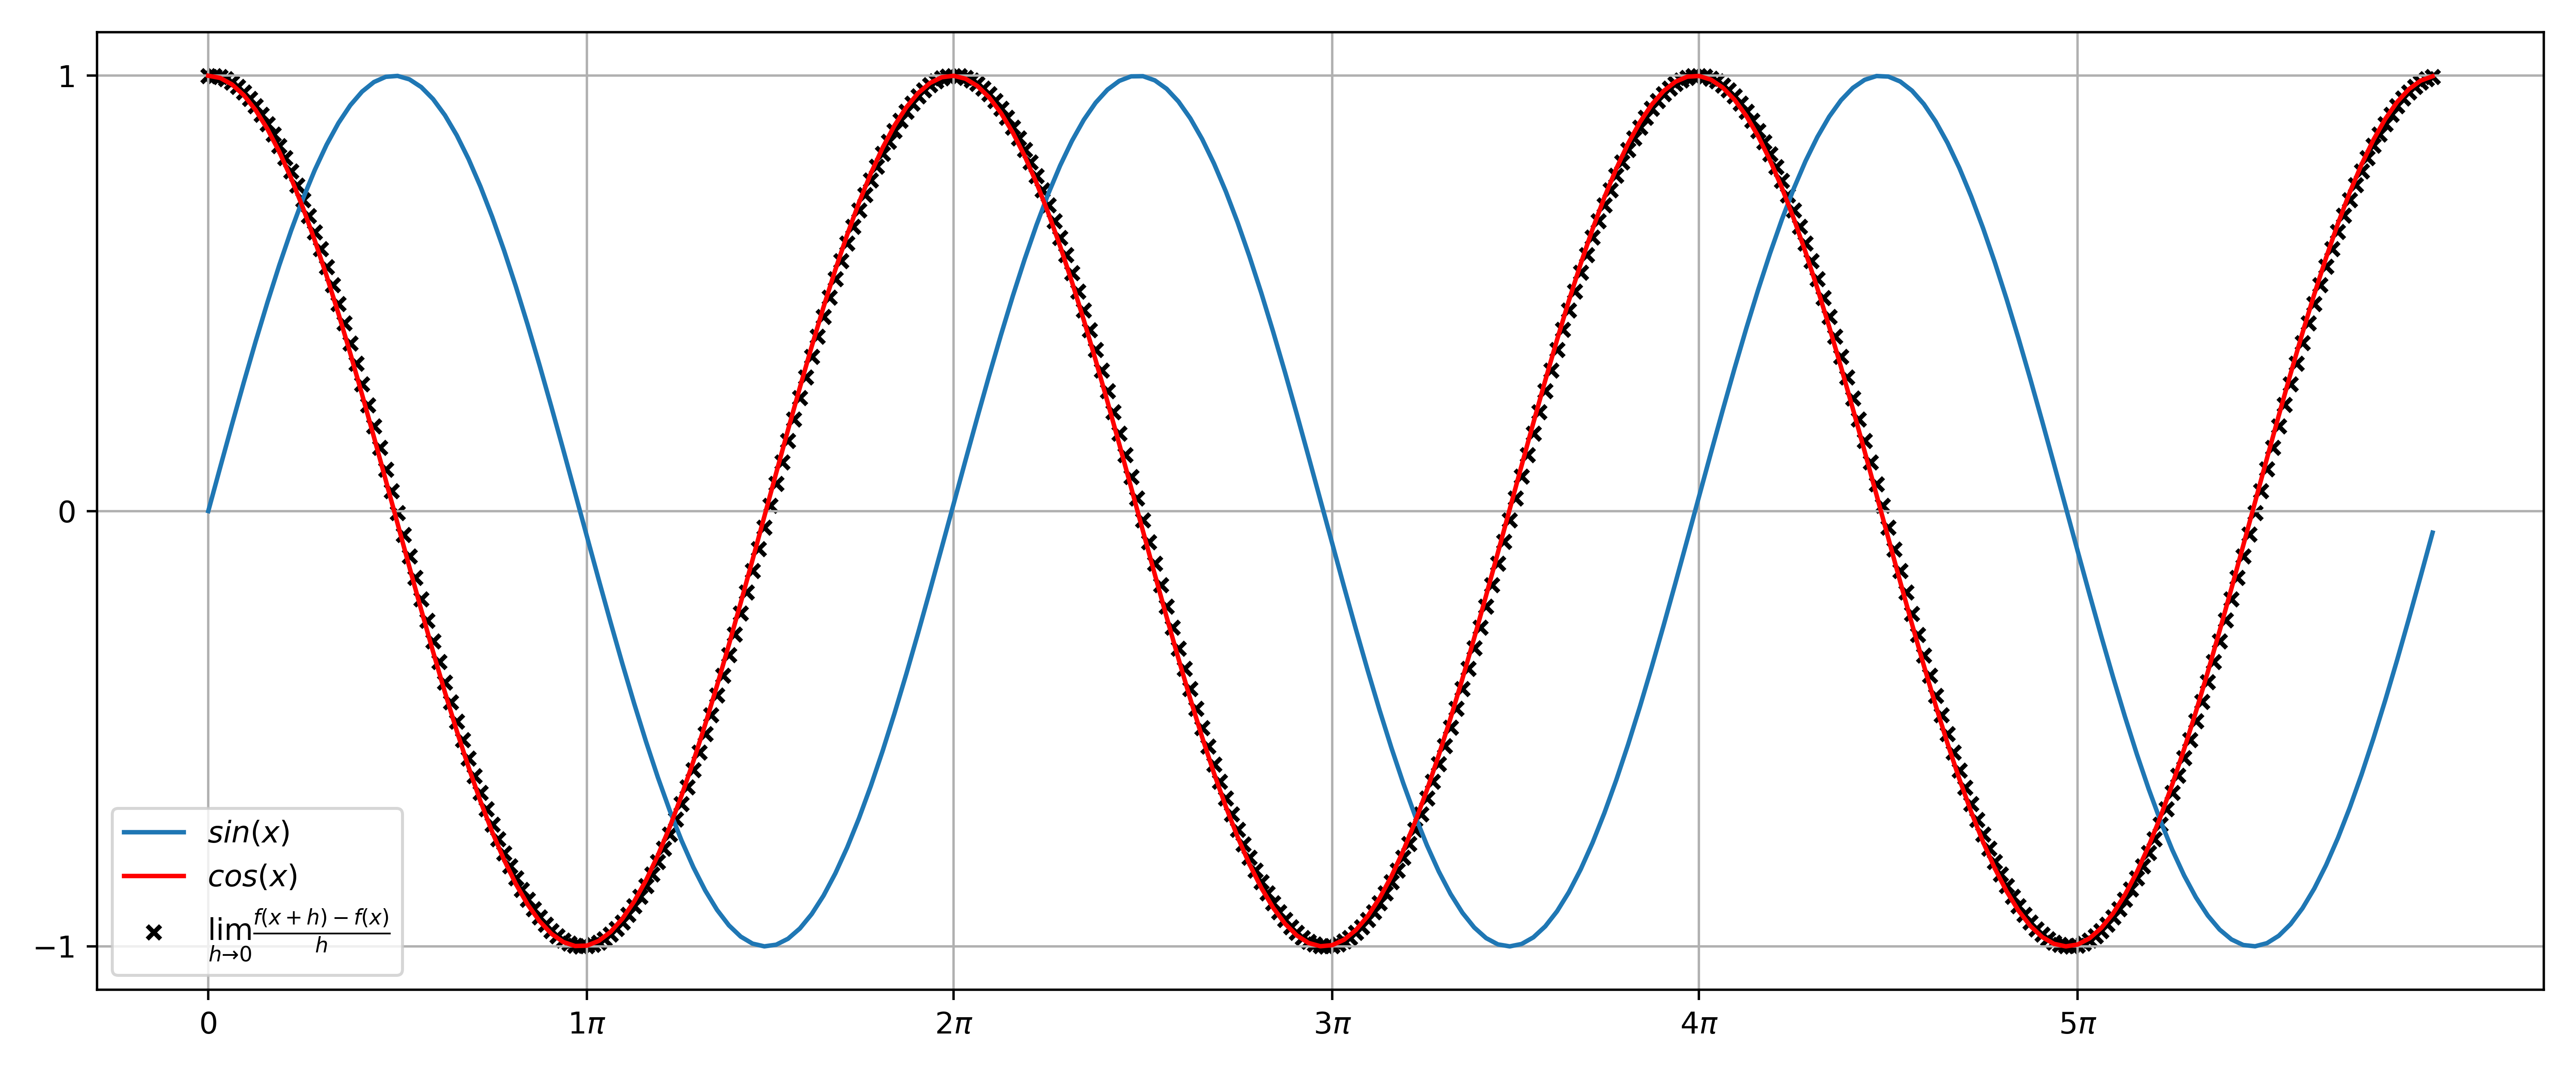
\includegraphics[width=6.5in]{plot.png}
    \caption{Numerical Derivative Plot (Black), Exact Derivative Plot (Red) of function $f(x)$ (Blue)}
    \label{fig:my_label}
\end{figure}

Noticeably, what we are plotting are \textit{the values of the slopes at every point x of the domain}, and thus, at the $x$ points where the minimum and maximum of $sin(x)$ are, the derivative or slope is 0, and thus we see the black crosses with height 0 at the corresponding $x$ points of these critical points of $f(x)$. The code for generating such plot is below.
\\

\begin{python}
# import sin and cos from math, matplotlib.pyplot and numpy
fig = plt.figure(figsize=(12, 5)); ax = fig.add_subplot(1,1,1)
h = 0.05
PI = 3.1416
cycles = 3
xs = [i for i in list(np.arange(0,PI*2 * cycles, 0.1))]
ys = [sin(x) for x in xs]; test = [cos(x) for x in xs]
dy = []; dx = []
for i in list(np.arange(0, PI*2 * cycles, h)):
    x = i - h
    x_plus_h = i
    lim = (sin(x_plus_h) - sin(x)) / h
    dy.append(lim)
    dx.append(i)
x_ticks = [0.0] + [x for x in xs if (x/PI) % 1 < 0.03 and (x/PI) > 1]
ax.plot(xs, ys, label=r"$sin(x)$")
ax.scatter(dx, dy, marker='x', color='black', s=20, label=r"$\lim_{h\to0} \frac{f(x+h) - f(x)}{h}$")
ax.plot(xs, test, label=r"$cos(x)$", color="red")
ax.set_xticks(x_ticks)
ax.set_yticks([-1, 0, 1])
ax.set_xticklabels(['0'] + [f"{int(t / PI)}" + r"$\pi$" for t in x_ticks[1:]])
\end{python}


% ////////////////////////////////////////////////////////////
%     Info ends
% ////////////////////////////////////////////////////////////
 
\end{document}
